\newpage
\section{Variationen des Graphen}
Die Aufgabenstellung legt die Topologie des planaren Graphen\footnote{Ein planarer Graph hat die Eigenschaft, dass er in der 2. Dimension dargestellt werden kann, ohne dass sich seine Kanten überschneiden.} fest, auf dem sich das Fahrzeug bewegen soll. Diese bleibt abgesehen von fehlenden Kanten oder blockierten Knotenpunkten fest. In einer 2D Darstellung können die Knotenpunkte in dem Rahmen verschoben werden, sodass die Topologie nicht verletzt wird. Das Ziel ist es, eine robuste Simulation zu erstellen, die mit möglichst vielen unterschiedlichen Variationen des Graphen funktioniert. Dafür wurde ein Tool entwickelt, das anhand eines Start-Graphen valide Variationen desselben entdeckt und diese abspeichert. 

\begin{table}[h!]
    \centering
    \begin{tabular}{|c|c|c|}
        \hline
        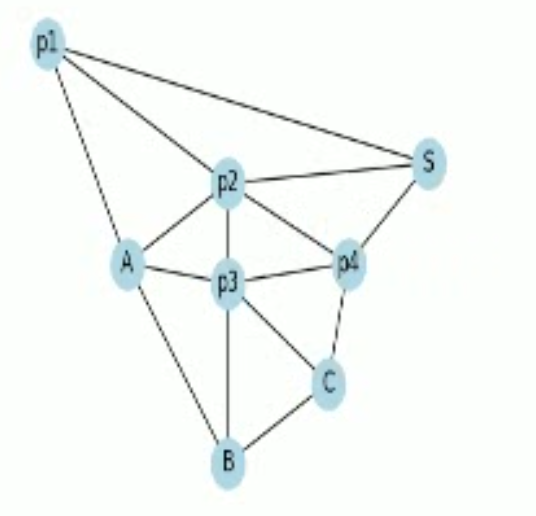
\includegraphics[width=5cm]{img/graphmorph/graph_morph1.png} & 
        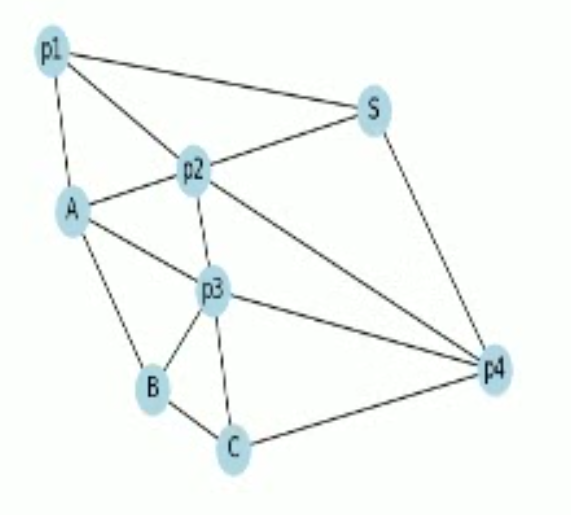
\includegraphics[width=5cm]{img/graphmorph/graph_morph2.png} & 
        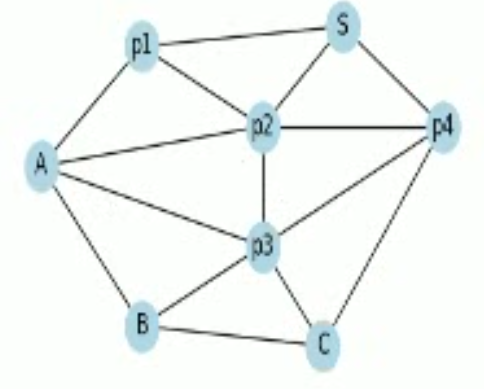
\includegraphics[width=5cm]{img/graphmorph/graph_morph3.png} \\
        \hline
    \end{tabular}
    \caption{Graph-Variationen des Ursprungsgraphen aus der Aufgabenstellung}
\end{table}

Die erstellten Graphen können für den Simulator, sowie die virtuelle Darstellung der Welt verwendet werden, siehe \ref{img:Übersicht Unreal Engine}

\begin{figure}[h!]
            \centering
            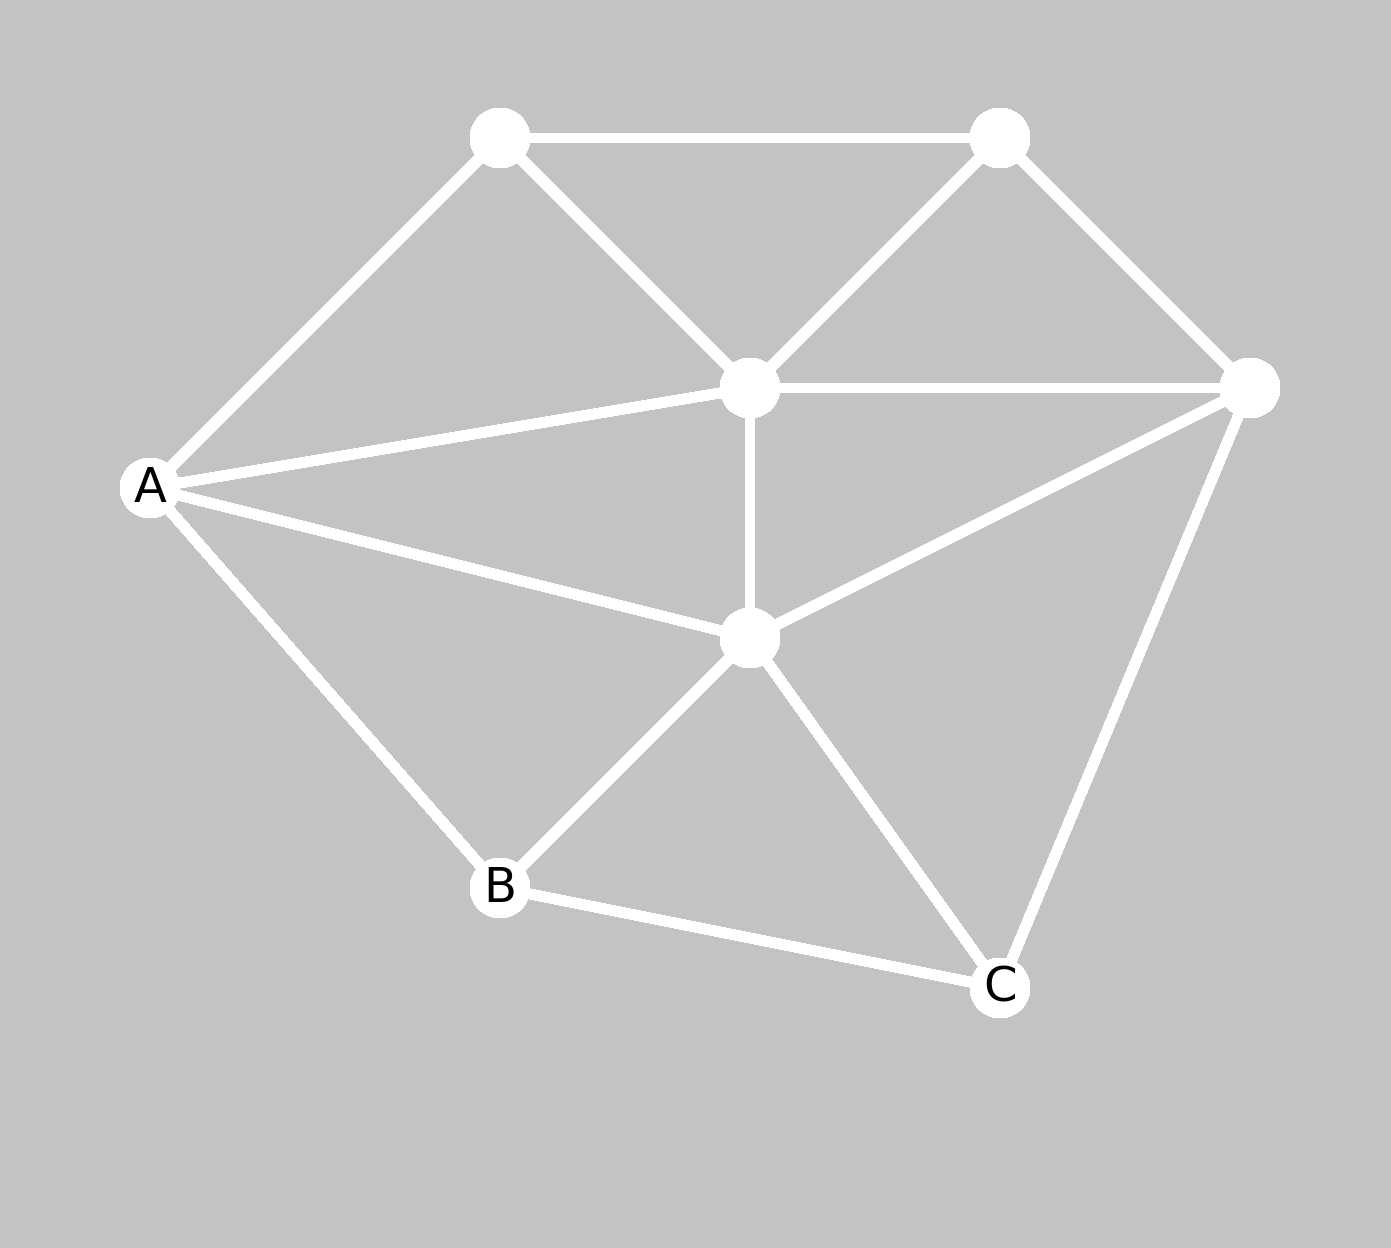
\includegraphics[width=0.5\textwidth]{img/graphmorph/graph_morph4.png}
            \caption{Export für den Gebrauch mit Unreal Engine}
        \label{img:Graph Export für Unreal Engine}
\end{figure}

